\documentclass[abstract=true]{scrartcl}

\usepackage[english]{babel}
\usepackage[utf8]{inputenc}
\usepackage[T1]{fontenc}
\usepackage{hyperref}
\usepackage{url}
\usepackage{booktabs}
\usepackage{amsfonts}
\usepackage{nicefrac}
\usepackage{microtype}
\usepackage{xcolor}
\usepackage{graphicx}
% \usepackage[numbers]{natbib}
\usepackage{lmodern}
\usepackage{geometry}
\usepackage{amsmath}
\usepackage{float}
\usepackage{textgreek}
\usepackage[backend=biber]{biblatex}
\usepackage{enumerate}
\geometry{bottom=40mm}
\usepackage[font=footnotesize]{caption}
\addbibresource{References.bib}

\author{
	Nabil Akbarazzima Fatih \\
	Mat-Nr: 3271528
}
\date{}
\title{Model Selection on Mixture Models Using the Akaike Information Criterion.}

\begin{document}
\maketitle
\vspace{5px}
\begin{center}
\Large
\textbf{Abstract}
\end{center}
The Expectation–Maximization (EM) algorithm is a popular tool in a wide variety of statistical settings, in particular in the maximum likelihood estimation of parameters when clustering using mixture models \cite{OHAGAN20123843}. But how to select a model on mixture models using the Akaike Information Criterion and to improve the results of the vanilla EM algorithm for fitting mixture models to the data? We will take a look on model selection according to the Akaike Information Criterion and the strategies to improve the results of the vanilla EM algorithm. The experiment with Expectation Maximization (EM) Algorithm is performed in the following two cases: the responsibilities parameters are initialized randomly and with K-means. The result shows that the Expectation Maximization (EM) Algorithm initialized with K-means performs better than the one initialized randomly.

\vspace{10px}
\section{Introduction}
%\section{Introduction, Background}

While maximum likelihood estimation can find the “best fit” model for a set of data, it doesn’t work particularly well for incomplete data sets. The more complex EM algorithm can find model parameters even if you have missing data \cite{stephanie}.
%\section{Introduction, Purpose/topic of review}
This paper presents how to perform model selection on mixture models using the Akaike Information Criterion, as well as the strategies to improve the results of the vanilla EM algorithm for fitting mixture models to the data.
%\section{Introduction, overview of content}
We implement the EM-algorithm for estimating the parameters of a mixture of k normal distributions $ \mathcal{N}(x;\mu_j,\sigma_j) $ with means $ \mu_j \in \mathbb{R}$  and standard deviations $ \sigma_j \in \mathbb{R} $.
We present the mathematical background of the Expectation Maximization and the Akaike Information Criterion. We underlay our results with plots.
%\end{titlepage}
\vspace{10px}
\section{Main analysis}
\subsection{Data}
In this paper we use three data sets: iris, blood pressure, and generated synthetic data set.
\begin{figure}[htbp]
	\begin{minipage}[t]{0.5\textwidth}
		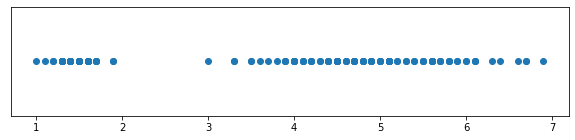
\includegraphics[width=0.9\textwidth]{images/iris_data.png}
		\vspace{-5px}
		\captionof{figure}{Petal lengths of iris data set}
	\end{minipage}
	\begin{minipage}[t]{0.5\textwidth}
 		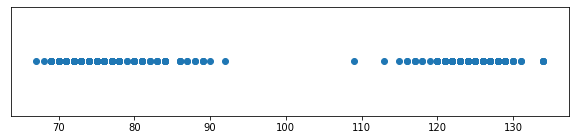
\includegraphics[width=0.9\textwidth]{images/bdp_data.png}
		\vspace{-5px}
		\captionof{figure}{Blood pressure values of blood pressure data set}
	\end{minipage}
	\noindent\makebox[\textwidth][c]{\begin{minipage}[c]{0.5\textwidth}
 		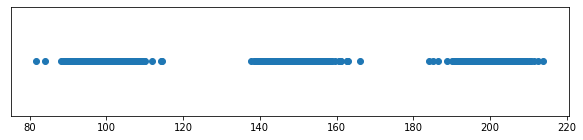
\includegraphics[width=0.9\textwidth]{images/sample_data.png}
		\vspace{-5px}
		\captionof{figure}{n data points randomly sampled from specified mixture of generated synthetic data set.}
	\end{minipage}}
\end{figure}
\subsection{Background}
First of all, we take a look at the needed mathematical background. In Expectation Maximization (EM) Algorithm for Gaussian Mixtures, we need to choose number of $k$ components and initialize parameter $\theta$ of mixture $f(x;\theta)$, then we need to repeat the following steps until termination:
\begin{enumerate}[Step 1:]
    \item Expectation (E): estimate responsibilities $\gamma(z_{ij})$ using current $\theta$
    \begin{equation}
    	\gamma(z_{ij}) = \frac{\pi_j N(x_i ; \mu_j, \Sigma_j)}{\sum_{l=1}^{k}\pi_l N(x_i ; \mu_l, \Sigma_l)}
    \end{equation}
    \begin{equation}
    	n_j = \sum_{i}^{n}\gamma(z_{ij})
    \end{equation}
    \item Maximization (M): re-estimate $\theta$ using current $\gamma(z_{ij})$
    \begin{equation}
    	\mu_j = \frac{1}{n_j} \sum_{i=1}^{n}\gamma(z_{ij})x_i
    \end{equation}
    \begin{equation}
    	\Sigma_j = \frac{1}{n_j} \sum_{i=1}^{n}\gamma(z_{ij})(x_i - \mu_j)(x_i - \mu_j)^T
    \end{equation}
    \begin{equation}
    	\pi_j = \frac{n_j}{n}
    \end{equation}
\end{enumerate}
We have the following equation for model selection according to Akaike Information Criterion (AIC):
\begin{equation}
    2|\hat{\theta}| - 2\mathcal{L_D}(\hat{\theta})
    \vspace{5px}
\end{equation}
Where $\mathcal{L_D}(\hat{\theta})$ is the log-likelihood of estimate $\hat{\theta}$ and $|\hat{\theta}|$ is the number of free parameters to estimate. A mixture of two normal distributions has 6 parameters
\begin{equation*}
    \theta = (\pi_1, \pi_2, \mu_1, \mu_2, \gamma_1, \gamma_2)
\end{equation*}
but only 5 free parameters. The reason is that we can infer $\pi_2$ from $\pi_1$ via $\pi_2 = 1 - \pi_1$. Thus, we only need to estimate $k-1$ instead of k mixing coefficients. The AIC uses this information when counting the number $|\hat{\theta}|$ of parameters to be estimated. For model selection, we choose a model with the smallest AIC value.
\subsection{Experiments}
We implemented the Expectation Maximization (EM) Algorithm for each of three data sets and for each $k \in \{1,...,15\}$ fit a model with $k$ components to the data. Then, Select the best model according to the Akaike Information Criterion. For default setting (Vanilla), the responsibilities (The method used to initialize the weights, the means and the precisions) are initialized randomly. The results of Vanilla Expectation Maximization (EM) Algorithm can be seen in the following plots:
\begin{figure}[H]			
	\begin{minipage}[t]{0.5\textwidth}
		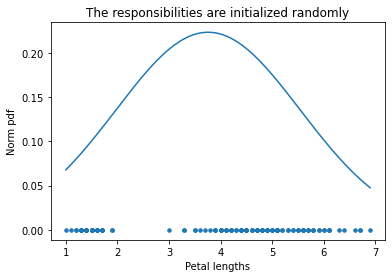
\includegraphics[width=\textwidth]{images/random_iris.png}
		\vspace{-20px}
 		\caption{AIC value: $599.10$ (Iris data set)}
	\end{minipage}
% 	\hspace{10px}
	\begin{minipage}[t]{0.5\textwidth}
 		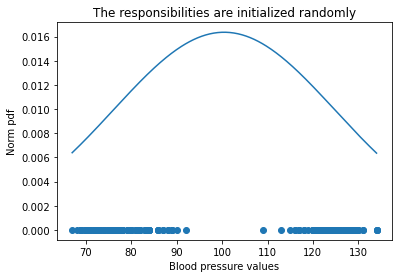
\includegraphics[width=\textwidth]{images/random_bdp.png}
 		\vspace{-20px}
 		\caption{AIC value: $2790.41$ (Blood pressure data set)}
	\end{minipage}
	\hspace{10px}
	\noindent\makebox[\textwidth][c]{\begin{minipage}[c]{0.5\textwidth}
 		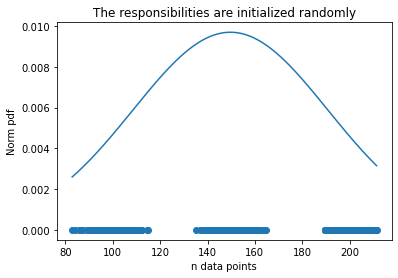
\includegraphics[width=\textwidth]{images/random_sample.png}
 		\vspace{-20px}
 		\caption{AIC value: $10276.95$ (Generated synthetic data
set)}
	\end{minipage}}
\end{figure}
Considering that in the results of Vanilla Expectation Maximization (EM) Algorithm if we initialized the responsibilities randomly, the performance of Expectation Maximization (EM) Algorithm looks poorly. So how can we improve the results of Expectation Maximization (EM) Algorithm? We changed the responsibilities parameter and initialized with K-means. We implement with the same steps like before for each of three data sets and for each $k \in \{1,...,15\}$ fit a model with $k$ components to the data, then select the best model according to the Akaike Information Criterion. The results of Expectation Maximization (EM) Algorithm after changing the responsibilities parameters can be seen in the following plots: 
\vspace{-10px}
\begin{figure}[H]
 	\begin{minipage}[t]{0.5\textwidth}
		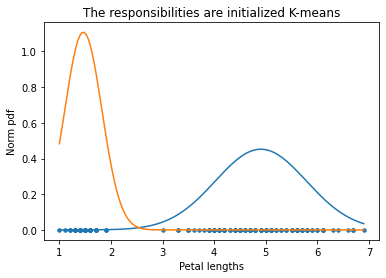
\includegraphics[width=\textwidth]{images/kmeans_iris.png}
		\vspace{-20px}
 		\caption{AIC value: $447.40$ (Iris data set)}
	\end{minipage}
% 	\hspace{10px}
	\begin{minipage}[t]{0.5\textwidth}
 		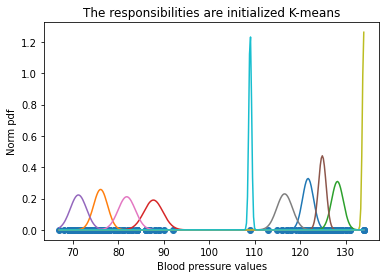
\includegraphics[width=\textwidth]{images/kmeans_bdp.png}
 		\vspace{-20px}
 		\caption{AIC value: $2173.55$ (Blood pressure data set)}
	\end{minipage}
	\hspace{10px}
	\noindent\makebox[\textwidth][c]{\begin{minipage}[c]{0.5\textwidth}
 		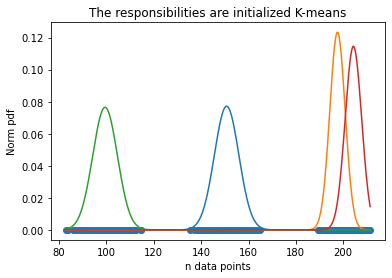
\includegraphics[width=\textwidth]{images/kmeans_sample.png}
 		\vspace{-20px}
 		\caption{AIC value: $8301.20$ (Generated synthetic data
set)}
	\end{minipage}}
\end{figure}
From the plots, we can conclude that Expectation Maximization (EM) Algorithm performs well after changing the responsibilities parameters to K-means. We found that Expectation Maximization (EM) Algorithm initialized with K-means improve the Expectation Maximization (EM) Algorithm's performance. 
\vspace{10px}
\section{Conclusion}
In our experiments we implemented the Expectation Maximization (EM) Algorithm and did a model selection on mixture models using the Akaike Information Criterion. The experiment results show that the Expectation Maximization (EM) Algorithm is sensitive to the responsibilities parameters. The Expectation Maximization (EM) Algorithm performs better with K-means than randomly initializing the responsibilities parameters. So in the future, we can consider using K-means for the responsibilities parameters for the strategies to improve the results of Expectation Maximization (EM) Algorithm.
\vspace{20px}
\printbibliography
\end{document}
